\documentclass[../../../doc/main]{subfiles}
\begin{document}
    \setcounter{chapter}{3}
    \setcounter{section}{2}
    \section{解説}\label{解説3}
    \begin{enumerate}
        \item [\kakkoichi] 円$C$を表す方程式は$x^2+(y-a)^2=1$である。$C$と$y=x^2$が接するときを考える。
            \begin{mawarikomi}{}{
                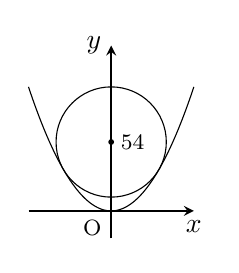
\begin{tikzpicture}[scale=.7]
                    \draw [semithick,-stealth] (-1.5,0) -- (1.5,0) node [below] {$x$};
                    \draw [semithick,-stealth] (0,-0.5) -- (0,3) node [left] {$y$};
                    \draw [samples=500,domain=-1.5:1.5] plot (\x,\x*\x);
                    \draw (0,5/4) circle(1);
                    \fill (0,5/4) circle(1.5pt) node [right] {\footnotesize $\bunsuu{5}{4}$};
                    \draw (0,0) node [below left] {\footnotesize O};
                \end{tikzpicture}
            }
            $x^2+(y-a)^2=1$と$y=x^2$を連立すると,
            \begin{align*}
                x^2+(x^2-a)^2=1 \Y (x^2)^2-(2a-1)x^2+a^2-1=0
            \end{align*}
            となるから,
            \begin{align*}
                (2a-1)^2-4(a^2-1)=0 \Y a=\bunsuu{5}{4}
            \end{align*}
            のときに接する。図と合わせて,求めるべき$a$の範囲は,
            \begin{align*}
                \boldsymbol{\bunsuu{5}{4}<a}\kotae
            \end{align*}
        \end{mawarikomi}
        \item [\kakkoni] $S$上の点Pの座標は$-\bunsuu{\pi}{2}\leqq\theta<0$を満たす媒介変数$\theta$を用いて,
            \begin{align*}
                \left\{
                    \begin{array}{l}
                        x=\cos{\theta} \\
                        y=a+\sin{\theta}
                    \end{array}
                \right.
            \end{align*}
            と表せる。この点Pでの$C$の接線の方程式は,
            \begin{align*}
                (\cos{\theta})\cdot x+(\sin{\theta})\cdot(y-a)=1~\sdots\sdots~\maruichi
            \end{align*}
            $\maruichi$ と$y=x^2$を連立すると,
            \begin{align*}
                (\cos{\theta})\cdot x+(\sin{\theta})\cdot(x^2-a)=1\quad\therefore\,\,(\sin{\theta})\cdot x^2+(\cos{\theta})\cdot x-a\sin{\theta}-1=0~\sdots\sdots~\maruni
            \end{align*}
            $\sin{\theta}\neq0$より,$\maruni$は$2$次方程式である。2つの解を$\alpha,\,\beta$とすると,解と係数の関係から,
            \begin{align*}
                \alpha+\beta=-\bunsuu{\cos{\theta}}{\sin{\theta}}\,,\quad\alpha\beta=-a-\bunsuu{1}{\sin{\theta}}
            \end{align*}
            $\maruichi$が$y=x^2$によって切り取られてできる線分の長さ$L_{\text{P}}$は,$\maruichi$の傾きが$-\bunsuu{1}{\tan{\theta}}$であることから,
            \begin{align*}
                L_{\text{P}}=\bunsuu{\emabs{\alpha-\beta}}{-\sin{\theta}}=\bunsuu{\sqrt{(\alpha-\beta)^2}}{\sqrt{\sin^2{\theta}}}=\bunsuu{\sqrt{(\alpha+\beta)^2-4\alpha\beta}}{\sqrt{\sin^2{\theta}}}=\sqrt{\bunsuu{1}{\sin^2{\theta}}\cdot\left(\bunsuu{1}{\tan^2{\theta}}+4a+\bunsuu{4}{\sin{\theta}}\right)}
            \end{align*}
            $t=\bunsuu{1}{\sin{\theta}}$とおくと,$t$の範囲は$t\leqq-1$で,$-\bunsuu{\pi}{2}\leqq\theta<0$から$t$の値と$\theta$の値は1対1に対応する。
            \begin{align*}
                {L_{\text{P}}}^2=t^2\left(t^2-1+4a+4t\right) \Y \bunsuu{d}{dt}{L_{\text{P}}}^2&=2t\left(t^2-1+4a+4t\right)+t^2\left(2t+4\right) \\
                &=2t\left\{2\left(t+\bunsuu{3}{2}\right)^2+4a-\bunsuu{11}{2}\right\}
            \end{align*}
            $L_{\text{Q}}=L_{\text{R}}$となる$S$上の相異なる$2$点Q,Rが存在するための必要十分条件は,$t$の関数${L_{\text{P}}}^2$が$t\leqq-1$で単調でないことである。それは,$2\left(t+\bunsuu{3}{2}\right)^2+4a-\bunsuu{11}{2}=0$が$t\leqq-1$の範囲に重解でない解をもつことと同値である。
            \begin{align*}
                4a-\bunsuu{11}{2}<0\quad\therefore\,\,a<\bunsuu{11}{8}
            \end{align*}
        よって,\kakkoichi の条件と合わせて,求めるべき$a$の範囲は,$\boldsymbol{\bunsuu{5}{4}<a<\bunsuu{11}{8}}$\kotae
    \end{enumerate}
\end{document}